\documentclass[a4paper]{article}

\usepackage{graphicx}
\usepackage{titlesec}
\usepackage{xcolor}
\usepackage{amsfonts}
\usepackage{wrapfig}
\usepackage{blindtext}
\usepackage{algorithm}
\usepackage{wrapfig}
\usepackage{algpseudocode}
\usepackage{multicol}
\usepackage{amssymb}
\usepackage{mathtools}
\usepackage{glossaries}
\setlength{\abovedisplayskip}{-10pt}  % Rimuove lo spazio prima delle equazioni
\setlength{\belowdisplayskip}{-10pt}  % Rimuove lo spazio prima delle equazioni



%\titlespacing*{\title}{0pt}{20pt}{200pt}
%\titlespacing*{\date}{0pt}{0ex}{0ex}
%\titlespacing*{\author}{0pt}{0ex}{0ex}

\titlespacing*{\section}{0pt}{0ex}{0ex}
\titlespacing*{\subsection}{0pt}{0ex}{0ex}
%\titlespacing\author{0pt}{0pt}{0pt}
%\titlespacing\date{0pt}{0pt}{0pt}
%\pagestyle{headings}
%\thispagestyle{headings}

\usepackage{graphicx} % Required for inserting images
\usepackage[a4paper, top=1cm, left=1.5cm, bottom=1.4cm, right=1.5cm]{geometry}

\title{
    \vspace{-1.5cm}
    \textbf{
        \large{
            CONVEX OPTIMIZATION AND ENGINEERING APPLICATIONS (Formulary)
   \vspace{-10ex}
        }
    }
}
\author{}
\date{}

\begin{document}
\maketitle
\thispagestyle{empty}
\vspace{0.15cm}
\subsection*{\underline{1. Introduction}}
\textbf{Standard form for optimization problems} $p^*=\min_{x} f_0(x) \ \text{s.t.} \quad f_i(x) \le 0, i=1,..., m$\\
where: $f_0: \mathbb{R}^n \to \mathbb{R}$ (\textbf{objective function}), $f_i: \mathbb{R}^n \to \mathbb{R}, $ (inequality constraints) \\
\textbf{Feasible set} $\mathcal{X} = \{x \in \mathbb{R}^n:\ f_i(x)\le 0\}$ \ |
\textbf{Optimal solution} $x^* \in \mathcal{X}: f(x^*)=p^*$ |
\textbf{Optimal value} $p^*$\\
\textbf{Equality constraints} $h_i(x)=0 \ i=1,...,p \ \iff \ h_i(x)\le 0, -h_i(x)\le 0$  --
\textbf{Optimal Set}  $\mathcal{X}_{opt} = \{x \in \mathcal{X} : f(x)=p^*\}$ \\
\textbf{Optimization problems in maximization form} $p^*=\max_{x} f_0 \iff -p^*=min_{x} \ -f_0(x) = min_{x} \ g_0(x)$\\
\textbf{$\varepsilon$-suboptimality of a solution} $x\in \mathbb{R}^n \ \iff \ p^* \le f_0(x) \le p^*+\varepsilon$

\subsection*{\underline{2. Vector, Projections, Functions, Gradients}}
\textbf{Vector} $x \in \mathbb{R}^n = [x_1 \quad x_2 \quad ... \quad x_n]^T$, $x_i\in\mathbb{R}$ -- 
\textbf{Sum} $x, y \in \mathbb{R}^n, x+y \iff x_i+y_i, \ i=1,...,n$\\
\textbf{Scalar multiplication} \ $\alpha \in \mathbb{R}, x \in \mathbb{R}^n, \ \alpha x \iff \ \alpha{x_i} \ i=1,...,n $\\
\textbf{Subspace} $\mathcal{V} \subseteq \mathcal{X}$ is a \textbf{subspace} $\iff$ $\forall x, y \in \mathcal{V}, \ \alpha{x}+\beta{y}\in\mathcal{V}$\\
$S=\{x^{(1)},...,x^{(n)}\}$, $\text{span}(S)=\{\alpha_1{x^{(1)}}+...+\alpha_n{x^{(n)}}, \ \alpha_i \in \mathbb{R}, \ i=1,...,n\}$\\
\textbf{Basis of a vector space} $B=\{b^{(1)}, ..., b^{(n)}\} \ \iff \ \text{span}(B)=\mathcal{X}$, $\forall x \in \mathcal{X}, x=\alpha_1{b^{(1)}+...+\alpha_n{b^{(n)}}}$, $\alpha_i\in\mathbb{R}$\\
\textbf{Direct sum of subspaces} $\mathcal{X,Y}\subseteq \mathbb{R}^n$, $\mathcal{X} \oplus \mathcal{Y}=\{x+y: \ x\in\mathcal{X}, y\in\mathcal{Y}\}$\\
\textbf{Affine set} $\mathcal{X}$ vector space, $\mathcal{V}\subseteq\mathcal{X}$ $\to$ affine set: $\mathcal{A}=\{x\in\mathcal{X}: x=x_0+v, \ v\in\mathcal{V}\}$, note that: $\dim_{\mathbb{R}}{\mathcal{A}}=\dim_{\mathbb{R}}{\mathcal{V}}$\\
\textbf{Line (1D-(affine set))} $L=\{x\in\mathbb{R}^n: \ x=x_0+v, \ v \in \text{span}(u), \Vert u \Vert_2=1\}$\\
\textbf{Norm} $\Vert \cdot \Vert: \mathbb{R}^n \to \mathbb{R}$ $\to$ $\Vert x \Vert \ge 0, \ \Vert x \Vert = 0 \iff x=0 $, 
$\Vert xy \Vert = \Vert x \Vert \Vert y \Vert$, $\Vert \alpha{x} \Vert =\vert \alpha \vert \cdot \Vert x \Vert$, 
$\Vert x+y \Vert \le \Vert x \Vert + \Vert y \Vert$ 
\textbf{$\ell_p$-norms} $\Vert x \Vert_p = \biggl(
    \sum_{i=0}^n{\vert x_i \vert}^p
\biggr)^{1/p}$, $p=2 \to $ Euclidean Distance, $p=1 \to$ Manahattan Distance, $p=\infty\to$ max $x_i$\\
\textbf{Inner Product}  $\langle x,y \rangle \ge 0$, $\langle x+y, z \rangle = \langle x,z \rangle + \langle y,z\rangle$, $\langle x,y\rangle=\langle y,x \rangle$, $\langle \alpha{x}, y \rangle=\alpha{\langle x,y \rangle }$, $\cos\theta=\frac{\langle{x,y}\rangle}{\Vert{x}\Vert_2 \Vert{y}\Vert_2 }$ \\
\textbf{Standard inner product} $x, y \in \mathcal{X}$, $\langle x, y \rangle = x^T{y}=\sum_{i=1}^n{x_i y_i}$, \textbf{Schwarz inequality} $\langle x, y \rangle \le \Vert{x}\Vert_2 \Vert{y}\Vert_2$,\\
 $\Vert x \Vert_2 = \sqrt{x^T x} = \sqrt{\langle x,x \rangle}$, $x \perp y \iff \langle x,y \rangle=0 \iff \cos\theta=0$\\
 $S=\{x^{(1)}, ..., x^{(n)}\}$ \textbf{mutually orthogonal} $\iff$ $\langle{x,y}\rangle = \begin{cases}
    0 \quad i{\ne}j\\
    \ne 0 \quad i= j
 \end{cases}$ \textbf{orthonormal} $\iff$ $\langle{x,y}\rangle = \begin{cases}
    1 \quad i{\ne}j\\
     0 \quad i= j
 \end{cases}$\\
\textbf{Vector $\perp$ Subspace} $\mathcal{S}\subseteq\mathcal{X}$, $x\in\mathcal{X}$, $x\perp\mathcal{S} \ \iff \langle{x,s}\rangle=0, \forall{s}\in\mathcal{S}$, $\mathcal{S}^{\perp}=\{x\in\mathcal{X}: \langle{x,s}\rangle=0, \forall{s}\in\mathcal{S}\}$\\
 \textbf{Orthogonal decomposition of a vector} $\forall{x}\in\mathcal{X}, x=x_1+x_2: \ x_1 \in \mathcal{S}, x_2 \in \mathcal{S}^{\perp}$ $\iff$ $\mathcal{X} = \mathcal{S} \oplus \mathcal{S}^{\perp}$\\
\textbf{Projections} $\Pi_{\mathcal{S}}(x)=\min_{y\in\mathcal{S}} \Vert y-s \Vert$ -- (\textit{\textsf{Projection Theorem}})
$
\begin{cases}
    x^*\in\mathcal{S} \ \text{is unique} \\
    (x-x^*) \perp \mathcal{S} \iff (x-x^*) \in \mathcal{S}^{\perp}
\end{cases}
$\\
\textbf{Functions}  $f:\mathbb{R}^n \to \mathbb{R}$ (function), $f: \mathbb{R}^n \to \mathbb{R}^m$ (map), \textbf{Domain of $f$}: $\text{dom}(f)=\{x\in\mathbb{R}^n: \ \Vert f(x) \Vert < \infty \}$\\
$\text{graph}(f)=\{(x,f(x))\in\mathbb{R}^{n+1}: \ x\in \mathbb{R}^n\}$, $\text{epi}(f)=\{(x,t)\in\mathbb{R}^{n+1}: \ x\in\mathbb{R}^n,t>=f(x)\}$\\
\textbf{Contour curves} $C_f(t)=\{x\in \mathbb{R}^n: f(x)=t, \  t\in\mathbb{R}\}$ -- \textbf{$\alpha$-sublevel set} $S_{\alpha}=\{x\in\mathbb{R}^n: \ f(x)\le t, \ t\in \mathbb{R}\}$       \\
$f$ is \textbf{linear} $\iff$ $f(\alpha x_1 + \beta x_2) = \alpha f(x_1) + \beta f(x_2)$, $\alpha, \beta \in \mathbb{R}$, $\tilde{f}$ is \textbf{affine} $\iff$ $\tilde{f}-x_0$ is linear\\
\textsf{any affine function can be written as: } $f(x)=a^T{x}+b$ where $a\in\mathbb{R}^n, \ b \in \mathbb{R}$, $b=f(0)$, $a_i = f(e_i)-b$, \\
\textbf{Hyperplane} $\mathcal{H}=\{x\in\mathbb{R}^n: \ a^T x = b\}$, $a\in \mathbb{R}^n$ (normal direction), 
$\mathcal{H}_{-} = \{x\in\mathbb{R}^n: \ a^T x \le b \}$, (open half-space) \\
$\mathcal{H}_{++}=\{x\in\mathbb{R}^n: \ a^T x > b\}$ (closed half-space)\\
\textbf{Gradient} Given $f:\mathbb{R}^n\to\mathbb{R}$ differentiable $\nabla{f}=\bigg[
    \frac{\partial f}{\partial x_1} \ \frac{\partial f}{\partial x_2}\ ... \ \frac{\partial f}{\partial x_n}
\bigg]^T$, $\nabla{f}(x_0)^T \cdot v $ (directional derivatives)\\
\textsf{the rate of variation is maximal} when $\nabla{f}(x_0)  \parallel v $ \textsf{minimal when} $\nabla{f}(x_0) \perp v$, moreover $\nabla{f}(x_0)\perp C_f(t) \ \forall x_0 \in \text{dom}(f)$

\subsection*{\underline{3. Matrices}}
\textbf{Matrix} $A\in\mathbb{R}^{m,n}$, $a_{ij}\in\mathbb{R}$ --- $AB_{ij}=R_i(A) \cdot C_j(B)$ (rows by column) --- $(AB)^T = B^T A^T$\\
An \textbf{affine map} $f=Ax+b$, $A\in\mathbb{R}^{m,n}, \ b \in \mathbb{R}^n$ (generalization of an \textbf{affine function})\\
\textbf{Subspaces associated with a matrix} $\begin{cases}
    \mathcal{R}(A) = \{Ax: x\in\mathbb{R}^n\} &\qquad \textsf{range of A}\\
    \mathcal{N}(A) = \{x \in \mathbb{R}^n: \ Ax=0\} &\qquad  \textsf{nullspace of A}\\
    \dim_{\mathbb{R}} {\mathcal{R}(A)}=\text{rank}(A), \ 1 \le \text{rank}(A) \le \min(m,n) &\qquad \textsf{rank of A}
\end{cases}$\\
\textbf{Fundamental thm. of linear algebra} For any $A\in\mathbb{R}^{m,n}$ $\begin{cases}
    \mathbb{R}^n\supseteq\mathcal{N}(A) \perp \mathcal{R}(A^T)\equiv\mathcal{N}(A)^{\perp} \iff \mathbb{R}^n = \mathcal{N}(A) \oplus \mathcal{R}(A^T)\\ 
    \mathbb{R}^m\supseteq\mathcal{R}(A) \perp \mathcal{N}(A^T)\equiv\mathcal{R}(A)^{\perp} \iff \mathbb{R}^m = \mathcal{R}(A) \oplus \mathcal{N}(A^T)\\
    \forall x \in \mathbb{R}^n, \ x=A^T{x}+\zeta, \ \zeta \in \mathcal{N}(A)\\
    \forall w \in \mathbb{R}^m, \ w=Ax+\xi, \ \xi \in \mathcal{N}(A^T)
\end{cases}$
\textbf{Singular matrix} $A \in \mathbb{R}^{n,n}$ is \textbf{singular} $\iff \det(A)=0$ $\iff$ $\mathcal{N}(A)\ne\{0\} \iff \text{rank}(A)\ne\min(m,n)$\\
\textbf{Inverse matrix} $A\in\mathbb{R}^{n,n}, \ \det(A)\ne 0$ $\exists A^{-1}\in\mathbb{R}^{n,n}: AA^{-1}=I_n$,
$(AB)^{-1} = B^{-1} A^{-1}$\\
\textbf{Similar matrices} $A,B \in \mathbb{R}^{n,n}$ are similar $\iff \ \exists P: B = P^{-1}A P$, $P$ is \textbf{non-singular} (columns: basis for $\mathbb{R}^{n,n}$) 
\textbf{Eigenvalues/Eigenvector} $u\in\mathbb{R}^{n,n}$ \textbf{eigenvector} for $A \ \iff$ $Au=\lambda u, \ u \ne0$, \\
$\lambda \to$ \textbf{\small{eigenvalue associated with $u$}}, \textbf{Eigenvalues} $\to$ {\tiny{roots of}} $p(\lambda)=\det(A-\lambda{I_n})=0$, \textbf{Eigenspace} $\to$ $\phi_i=\mathcal{N}(A-\lambda_i{I_n})$\\
\textbf{\underline{Algebraic Multiplicity}} $\nu_i$ (multiplicity of the root of $p(\lambda)$) \textbf{\underline{Geometric Multiplicity}} $\mu_i=\dim_{\mathbb{R}}(\phi_i)$ $\longrightarrow$ $\nu_i \le \mu_i$
\textbf{Diagonalizable matrices (thm.)} $\lambda_i, \ i=1,...,k \le n$ (distinct eigenvalues of A), $U^{(i)}=[u_1^{(i)}\quad\dots\quad{u_{\nu_i}^{(i)}}]$ the eigenvector wrt $\lambda_i$, \textbf{if $\nu_i=\mu_i, \  i=1,...,k$}, $U=[U^{(1)}\quad\dots\quad{U^{k}}]$ is \textbf{invertible} and $A=U{\Lambda}U^{-1}$, $\Lambda=diag(\lambda_1{I_{\mu_1}}, ...,\lambda_k{I_{\mu_k}})$\\
\textbf{Matrix norms} ...is a function $f:\mathbb{R}^{m,n}\to\mathbb{R}$ --- additional property $\underline{f(AB)\le{f(A) f(B)}}$ \textbf{sub-multiplicativity}\\
\textbf{Frobenius norm} (extension of $\ell_2$-norm) $\Vert A \Vert_F = \sqrt{\text{trace}(A^T A)} = \sqrt{
    \sum_{j=1}^m {\sum_{i=1}^n { a_{ij}^2}}} = \sqrt{\sum_{i=1}^n \lambda_i(A^T A)}$ \\
\textbf{Operator norms} (max input-output gain of $y=Au$) $\Vert A \Vert_p \doteq \max_{u{\ne}0}\frac{\Vert Au \Vert_p}{\Vert u \Vert_p}=
\max_{\Vert{u}\Vert_p=1}{\Vert Au \Vert_p}$ ($\ell_p$-induced norms)\\
$\Vert A \Vert_1 = \max_{j=1,...,m}{\sum_{i=1}^n \vert a_{ij} \vert}, \
\Vert A \Vert_\infty = \max_{i=1,...,m}{\sum_{j=1}^n \vert a_{ij} \vert}, \
\Vert  A \Vert_2 = \sqrt{\lambda_{\text{max}} (A^T A)} $ {\tiny{(see variational characterization)}}\\
\textbf{Spectral radius} $A\in\mathbb{R}^{n,n}$ $\rho(A)\doteq\max_{i=1,...,n} \vert \lambda_i(A) \vert$ --- $\rho(A)\le\min(\Vert A \Vert_1, \Vert A \Vert_\infty)$
\subsection*{\underline{4. Symmetric Matrices and SVD}}
$A\in\mathbb{R}^{n,n}$ is \textbf{symmetric} if $AA^T=I_n \iff A^{-1}=A^T$, $\mathbb{S}^n$ is the subspace of \textbf{symmetric matrices} $n\times{n}$ \\
\textbf{Examples:} (Hessian matrix given $f:\mathbb{R}^2\to\mathbb{R}$) $H=\begin{bmatrix}
    \frac{\partial{f}}{\partial{x_1^2}}&\frac{\partial{f}}{\partial{x_1{x_2}}}\\
    \frac{\partial{f}}{\partial{x_2{x_1}}}&\frac{\partial{f}}{\partial{x_2^2}}
\end{bmatrix}$, (quadratic function) $q(x)=\frac{1}{2}x^T{H}x+c^T{x}+d$\\
\textbf{Quadratic form} Given $A\in\mathbb{S}^n, \ \forall x \ne 0$ the function $q(x)=x^T A x$ is a \textbf{quadratic form associated with A}\\
\textbf{Spectral theorem} Given $A\in\mathbb{S}^n$ it holds that: $\lambda_i\in\mathbb{R}, \ i=1,...,n$, exists $U=[u_1\quad\dots\quad{u_n}]$ orthogonal and $A=U\Lambda{U^T}=\sum_{i=1}^{n}{\lambda_i{u_i}u_i^T}$, $\Lambda=diag(\lambda_1, ..., \lambda_n)$. I can sort them $\lambda_{max}(A)=\lambda_1 \ge \lambda_2 \ge \dots \ge \lambda_n=\lambda_{min}(A)$\\
\textbf{Rayleigh quotient} given $A\in\mathbb{S}^n$, we can define $\forall x \in \mathbb{R}^n$ the quantity $r(x)=\frac{x^T{A}x}{x^T{x}}$ (Rayleigh quotient)\\
\textbf{Theorem} For any $A\in\mathbb{S}^n, \ \forall x \ne 0$, $\lambda_{max} \le r(x) \le \lambda_{min}$, where 
$\begin{cases}
    \lambda_{max}(A)=\max_{\Vert x \Vert_2=1} {x^T A x}&(x^*=u_1)\\
    \lambda_{min}(A)=\min_{\Vert x \Vert_2=1} {x^T A x}&(x^*=u_n)\\
\end{cases}$\\
\textbf{...on the $\ell_2$-induced norm} (by using the definition of operator norm and $\ell_2$-norm) $\frac{\Vert Ax \Vert_2^2}{\Vert x \Vert_2^2}=\frac{(Ax)^T{(Ax)}}{x^T{x}} = \frac{x^T{(A^T{A})x}}{x^T{x}}$ that is the Rayleigh quotient of $A^T{A}\in\mathbb{S}^n$ from the theorem follows that $\Vert A \Vert_2 = \max_{\Vert x \Vert \ne 0} r_{\small A^T A}(x)=\sqrt{\lambda_{max}(A^T A)} \quad \square$ \\
Given a symmetric matrix, it is said to be $\begin{cases}
    \textbf{Positive definite} (A\succ0)& \forall x\in \mathbb{R}^n, x^T{A}x>0 \iff \lambda_i>0,\ i=1,...,n\\
    \textbf{Positive semidefinite} (A\succeq 0)&\forall x\in \mathbb{R}^n, x^T{A}x\ge0 \iff \lambda_i\ge0,\ i=1,...,n\\
    \textbf{Negative definite}(A\prec 0)&\forall x\in \mathbb{R}^n, x^T{A}x<0 \iff \lambda_i<0,\ i=1,...,n\\
    \textbf{Negative semidefiite} (A\preceq 0)&\forall x\in \mathbb{R}^n, x^T{A}x\le0 \iff \lambda_i\le0,\ i=1,...,n\\
\end{cases}$\\
\textbf{Matrix square-root} $A\succeq0 \Rightarrow \exists{B}: \ A = B^2$, $B=A^{1/2}$ is the \textbf{matrix square-root}\\
\textbf{Cholesky decomposition} $A\succ0 \iff \exists B: A=B^T{B}$, such a $B$ can be computed as: $B=U\Lambda^{1/2}U^T$, where $U$ comes from the spectral decomposition and $\Lambda^{1/2}=diag(\sqrt{\lambda_1}, ..., \sqrt{\lambda_n})$\\
\textbf{\underline{SINGULAR VALUE DECOMPOSITION(SVD)}} (It holds for any matrix $A\in\mathbb{R}^{m,n}$, $A^T{A}$ is very important!)\\
\textbf{Theorem} Given $A\in\mathbb{R}^{m,n}$, it can be written as: $A=U\tilde{\Sigma}V^T$, $U\in\mathbb{R}^{m,m}$, $V\in\mathbb{R}^{n,n}$ are \textit{orthogonal matrices} while $\tilde{\Sigma}=\begin{bmatrix}
    \Sigma&0_{r,n-r}\\
    0_{m-r,r}&0_{m-r,n-r}
\end{bmatrix}, \Sigma = diag(\sigma_1, ..., \sigma_r), \ \sigma_1 \ge \sigma_2 \ge ... \ge \sigma_n \ge0$ are the \textbf{singular values}, $U=[u_1,...,u_r]$ are the \textbf{left singular vector}, $V=[v_1, ..., v_r]$ are the \textbf{right singular vector}.\\
\textbf{SVD (compact form)} $A=U_r\Sigma V_r=\sum_{i=1}^r{(\sigma_i u_i v_i^T)}$, moreover $\begin{cases}
    \sigma_i^2 = \lambda_i({A^T}{A}), \sigma_1^2 = \lambda_{max}({A^T A})\\
    u_i \ \textbf{eigenvectors of} \ AA^T\\
    v_i \ \textbf{eigenvectors of} \ A^T{A}
\end{cases}$\\
\textbf{Properties of SVD} We can redefine some properties by using SVD $\begin{cases}
    rank(A)=r\\
    \mathcal{N}(A)=\mathcal{R}\bigl([v_{r+1}\dots v_n]\bigr), \ \mathcal{R}(A)=\mathcal{R}\bigl([u_1\dots u_r]\bigr)\\
    \Vert A \Vert_F^2 = \sum_{i=1}^r {\sigma_i^2},
    \Vert A \Vert_2^2 = \lambda_{max}(A^T A) = \sigma_1^2\\
    \Vert A \Vert_* = \sum_{i=1}^r \sigma_i \ \textbf{nuclear norm}
\end{cases}$\\
\textbf{Moore-Penrose pseudo-inverse} $A^\dagger=V\tilde{\Sigma}^\dagger{U^T}$ (or in compact form) $A^{\dagger}=V_r\Sigma^{-1} U_r^T$, (full column) $A^{\dagger}=(A^T A)^{-1}A$
\textbf{Condition number} \textsf{How close is $A$ to be singular?} $\kappa(A)=\frac{\sigma_1}{\sigma_n}$ the larger $\kappa$ the closest $A$ to be singular.\\
\textbf{Low rank approximation} $A_k = \arg\min_{A_k\in\mathbb{R}^{m,n},\\  rank(A_k)=k}{\Vert A-A_k \Vert_F^2}=
\sum_{i=1}^\mathbf{k} {(\sigma_i u_i v_i^T)}$\\
\textbf{Ratio of the total variance in $A_k$} is the quantity $\eta_k  =  \frac{\Vert A_k \Vert_F^2}{\Vert A \Vert_F^2}= \frac{\sigma_1^2+...+\sigma_k^2}{\sigma_1^2+...+\sigma_n^2}$ is useful a graph $k$ vs $\eta_k$ to choose properly $k$ --- \textbf{Norm approximation error} $e_k=\frac{\Vert A-A_k \Vert_F^2}{\Vert A \Vert_F^2}=1-\eta_k$ \\
\textbf{Application: \underline{Principal component Analysis (PCA)}} I collect in a matrix $X\in\mathbb{R}^{n,m}$ by columns $m$ samples characterized by $n$ features. $\tilde{X}=[x_1-\bar{x}\ ...\ x_m-\bar{x}], \ \bar{x}=\frac{1}{m}\sum_{i=1}^m {x_i} \ \text{(baricenter)}.  \ x_i \in \mathbb{R}^n$\\
\textbf{I want a direction $z\in\mathbb{R}^n$ along which the projections of the centered data have the maximal variance.}\\
\textbf{Ingredients}: $\begin{cases}
    \textsf{projection on} \ z & \alpha_i=\tilde{x}_i^T{z}, \ i=1,...,m\\
    \textsf{variance}& \frac{1}{m} \sum_{i=1}^{m}{\alpha_i}^2=\sum_{i=1}^{m}{z^T \tilde{x}_i \tilde{x}_i^T{z}}=z^T\tilde{X}\tilde{X}^T{z} 
\end{cases}$\\
Problem to solve: $\qquad\underset{z\in\mathbb{R}^n}{\text{max}}\ {z^T \tilde{X}\tilde{X}^T z}$\ , 
$\tilde{X} \underset{\textsf{SVD}}{=}U_r\Sigma{V_r}^T, \ \tilde{X}\tilde{X}^T=U_r\Sigma^2{U_r}^T$ (spectral decomposition)\\
from the theorem: $z=u_1$ (\textbf{first principal component}) $\to$ the $i$-th principal component $\iff$ $i$-th row of $U$ from SVD. $U_k \in \mathbb{R}^{n,k}$ (first $k$ principal components, columns of $U$) $\longrightarrow$ I choose $k$ according to $\eta_k$, then: $x=\bar{x}+U_k{z},
\ z\in\mathbb{R}^k$ (zero-mean random factors). \textbf{Result:} we are using $z\in\mathbb{R}^k$, instead of $x\in\mathbb{R}^n$, $k<n$ to represent our data. $\square$\\

\subsection*{\underline{5. Least Squares (LS)}}
\textbf{Applications:} $\begin{cases}
    \textsf{approximation for a "fat" system of equations}\\
    \textsf{polynomial approximation/regression}
\end{cases}$ {\large{$y = Ax \underset{\text{relax}}{\longrightarrow} y \simeq Ax$}},  \textbf{residuals} $r(x) = Ax-y$\\
\textbf{Objective:} find an $x$ such that the squared-residuals are "small" 
$f_0(x) = \sum_i {r_i^2(x)} =\sum_i {(a^T x - y_i)^2} = \Vert Ax-y \Vert_2^2$\\
\textbf{Least Squqres problem: }    $\underset{x\in\mathbb{R}^n}{\text{min}} \ {\Vert Ax-y \Vert_2^2}$ (unconstrained)--- 
\textbf{Solution} we have to find the roots of $\nabla{f_0}(x)=0$\\
\textbf{Rewriting of the $f_0$} $\Vert Ax-y \Vert_2^2 = x^T{Q}x-2b^T{x}+c$, $Q=A^T A\succ0, \ b=A^T y, \ c=\Vert{y}\Vert_2^2$\\
$\nabla{f_0}(x)=0\iff Qx=b\iff \mathbf{A^T A x = A^T y}$ (normal equations) $x=(A^T A)^{-1} A^T y$ (for full column $A$)\\
\textbf{Geometric interpretation (projections)} LS problem can be recasted as: $\min_{\tilde{y}\in\mathcal{R}(A)}{\Vert \tilde{y} - y \Vert_2^2}$\\
You know from the projection theorem that: (i) $\tilde{y}\in\mathcal{R}(A)$, (ii) $(\tilde{y}-y) \perp \mathcal{R}(A) \iff (\tilde{y}-y)\in \mathcal{N}(A^T)\iff A^T{(\tilde{y}-y)}=0 \iff A^T{(Ax-y)}=0  \iff A^T A x = A^T y$ (normal equations)\\
\textbf{Variants for the LS problem} $\begin{cases}
    \textsf{LS+\textbf{Equality constraints}}& \min_x {f_0} \ \text{s.t.} \  Cx=d \to x=\bar{x}+Nz, \  \text{span($N$)=$\mathcal{N}(C)$}\\
     & \min_x {\Vert \bar{A}x-\bar{y}\Vert_2^2}, \ \bar{A}=AN,  \ \bar{y}=y-A\bar{x}\\
    \textsf{LS+\textbf{weighted residuals}}& f_0=\sum w_i r_i^2(x) = \Vert W(Ax-y) \Vert_2^2, \ W=diag(w_1,...,w_n)\\
     & \min_x \Vert A_w x -y_w \Vert_2^2, \ A_w = WA, \ y_w = Wy\\
    \textsf{LS+\textbf{$\ell_2$-regularization}}&\min_{x} {\Vert Ax-y \Vert_2^2} + \gamma\Vert x \Vert_2^2, \ 
    {\small \Bigg\Vert 
        \begin{bmatrix}
            a\\b
        \end{bmatrix}
     \Bigg\Vert}_2^2 = \Vert a \Vert_2^2 + \Vert b \Vert_2^2\\
      & \min_x {\Vert{\tilde{A}x-\tilde{y}}\Vert}, \tilde{y} = [y\quad{0_n}]^T, \ \tilde{A} = [A\quad \sqrt{\lambda}{I_n}]^T
\end{cases}$

\subsection*{\underline{6. Convexity: sets and functions}} 
Given $P=\{x^{(1)}, x^{(2)}, ..., x^{(m)}\}$, $\begin{cases}
    \textbf{linear combination} & \lambda_1 x^{(1)}+\lambda_2 x^{(2)}+...+\lambda_m x^{(m)} , \lambda_i \in \mathbb{R}\\
    \textbf{convex combination} & \lambda_i \in \mathbb{R}, \lambda_i \ge 0, \sum \lambda_i = 1
\end{cases}$\\
\textbf{Well-known subspaces} $\begin{cases}
    \textsf{linear hull}&\textbf{subspace with all linear combinations}\\
    \textsf{affine hull}&\text{aff}(P), \ \lambda_i \in \mathbb{R},\ \sum \lambda_i = 1\\
    \textsf{convex hull}&\text{co}(P)\ \textbf{subspace with all convex combinations}\\
    \textsf{conic hull}&\text{conic}(P) \ \lambda_i \in \mathbb{R}, \lambda_i \ge 0
\end{cases}$\\
\textbf{\underline{CONVEX SETS}} $\mathcal{C}\subseteq\mathbb{R}^n$ \textbf{convex} $\iff \forall x,y \in \mathcal{C} \to$ the segment joining $x$ and $y$ lies in $\mathcal{C}$. More formally, a convex combination of any two points falls within $\mathcal{C}$...\\
$\underbrace{\forall x,y, \ \lambda \in [0,1], \ x,y \in \mathcal{C} \to \ \lambda x + (1-\lambda{y})\in\mathcal{C}}_{\textsf{convex set}}$, $\quad\underbrace{x\ne{y}, \lambda \in (0,1), \lambda{x}+(1-\lambda){y} \in \text{relint}(C) }_{\textsf{strictly convex set}}$\\
\textbf{Cone and convex cone} Given $\mathcal{C}\subseteq\mathbb{R}^n$ is a \textbf{cone} $\iff x\in\mathcal{C} \to \alpha{x}\in\mathcal{C}, \ \alpha>0$ --- $\mathcal{C}$ also convex $\to$ \textbf{convex cone}\\
\textbf{Operations preserving convexity}  $\begin{cases}
    \textsf{Intersections with convex sets}& \mathcal{C}_1, ..., \mathcal{C}_n \ \text{convex } \to \mathcal{C}=\bigcap_{i=1}^n{\mathcal{C}_i} \ \textbf{is convex}\\
    \textsf{Affine transformations}&f(x)=Ax+b, \mathcal{C} \ \text{cvx} \to  f(C)=\{f(x): \ x\in\mathcal{C}\}\ \text{cvx}
\end{cases}$\\
\textbf{Supporting Hyperplane} $\underset{\overline{\textbf{Thm}.:\  \text{exists} \ \text{separating} \ \mathcal{H} \ \text{for} \ \mathcal{C}\ \text{at}\ z}}{\text{Given} \ \mathcal{C} \ \text{convex set}, z\in\partial\mathcal{C}}$, $\mathcal{H}$ \textbf{supporting hyperplane} $\iff \ z \in \mathcal{H}$ and $\mathcal{C} \subseteq \mathcal{H}_{-}$\\
\textbf{Separating Hyperplane} $\underset{\textbf{Thm.:}\ \mathcal{C}_1 \cap \mathcal{C}_2=\emptyset \ \text{exists} \ \text{sep.}\ \mathcal{H}}
{\underline{\text{Given}\ \mathcal{C}_1, \mathcal{C}_2 \ \text{convex sets}}}$ the hyperplane $\mathcal{H}: \begin{cases}
    \textsf{\textbf{separates} the sets}&\mathcal{C}_1 \subseteq \mathcal{H}_{-}, \mathcal{C}_2 \subseteq \mathcal{H}_+\\
    \textsf{\textbf{strictly separates} the sets}&\mathcal{C}_1 \subseteq \mathcal{H}_{--}, \mathcal{C}_2 \subseteq \mathcal{H}_{++}\\
\end{cases}$\\
\textbf{\underline{CONVEX FUNCTIONS}}\\
$f:\mathbb{R}^n \to \mathbb{R}$ is $\begin{cases}
\textbf{convex} \iff \textbf{(i)} \ \text{dom}(f) \ \text{convex}, \textbf{(ii)} \ x,y\in\text{dom}(f), \ \lambda \in [0,1]
\to f(\lambda{x}+(1-\lambda){y})\le\lambda{f(x)}+(1-\lambda)f(y)\\
\textbf{strictly convex} \iff  x,y\in\text{dom}(f), \ \lambda \in [0,1]
\to f(\lambda{x}+(1-\lambda){y})<\lambda{f(x)}+(1-\lambda)f(y)\\
\textbf{strongly convex}\iff \exists m >0: \ \tilde{f}(x)=f(x)-\frac{m}{2}\Vert{x}\Vert_2^2 \ \text{is convex} \underset{\text{imply}}{\to} \ \text{strictly convex}\\
\end{cases}$ \\
\textbf{Properties} $f$ convex(cvx) $\Leftrightarrow$ $\text{epi}(f)$ is cvx --- $f$ cvx $\Rightarrow$ $S_\alpha$ ($\alpha$-sublevel set) is convex $\forall \alpha$ ---
$f$ str. cvx $\substack{\Rightarrow\\\nLeftarrow} \ S_\alpha$ str. cvx\\
$f,g$ strictly convex $\Rightarrow$ $f+g$ strictly convex --- $f$ convex, $g$ strongly convex $\Rightarrow$ $f+g$ strongly convex\\
$h,g$ convex, $g$ non decreasing $\Rightarrow$ ${h}\circ{g}$ cvx --- $g$ concave, $h$ convex non-increasing $\Rightarrow$ ${h}\circ{g}$ cvx\\
\textsf{\small{Non-negative linear combinations}} {\small{
    $f_i:\mathbb{R}^n\to\mathbb{R}, \ i=1,...,m$ convex $\Rightarrow$ $f=\sum_{i=1}^m{\alpha_i f_i},\ \alpha_i\ge0$ is convex over $\cap
    _i{\text{dom}(f_i)}$
}}\\
\textsf{\small{Affine variable transformation}} {\small{
    $f:\mathbb{R}^n\to\mathbb{R}, \ g(x)=f(Ax+b)$ is convex 
}}\\
\textbf{Conditions for convexity} $\begin{cases}
    \underset{f \ \text{differentiable}}{\textsf{\textbf{First-order condition}}}& f \ \text{convex} \ \iff \ \forall{x,y}\in\text{dom}(f), \ f(y)\ge f(x)+\nabla{f(x)}^T(y-x)\\
    \underset{f \ \text{twice differentiable}}{\textsf{\textbf{Second-order condition}}}& \begin{cases}
        f \ \text{convex} \ \iff \ \nabla^2{f(x)}\succeq0 \ \forall x \in \text{dom}(f)\\
        f \ \text{strictly convex} \substack{\Leftarrow\\\nRightarrow} \ \nabla^2{f(x)}\succ0\\
        f \ \text{strongly convex} \ \exists{m}: \ \nabla^2{f(x)}\succ{m{I}}, \ \forall x \in \text{dom}(f)
    \end{cases}\\
    \textsf{\textbf{Restriction to a line}}& f \ \text{convex} \ \iff \underbrace{g(t)=f(x_0+tv)}_{\textsf{restriction of $f$ to a line}}, \ x_0,v\in\mathbb{R}^n, \ t \in \mathbb{R} \ \text{is convex}
\end{cases}$\\
\textbf{Pointwise maximum} $f_\alpha(x)$ convex and $\alpha\in\mathcal{A}$, $\mathcal{A}$ compact set(closed and bounded), $f(x)=\max_{\alpha\in\mathcal{A}}{f_\alpha(x)}$ is convex\\
\textbf{Jensen's inequality} Given $f:\mathbb{R}^n\to\mathbb{R}$ convex and $z\in\mathbb{R}^n$ a random variable such that $p\{z\in\text{int}\ {\text{dom}(f)}\}=1$ it holds that: $f(\mathbb{E}[z])\le\mathbb{E}[f(z)]$. \textbf{Case $z$ discrete R.V.} $p(z=x^{(i)})=\theta_i, \ i=1,...,m$, $\sum_i{\theta_i}=1$, $\theta_i\ge0$ $\Rightarrow$ $f\big(\sum_i{\theta_i{x^{(i)}}}\big)\le\sum_i{\theta_i{f\big(x^{(i)}\big)}}$\\

\subsection*{\underline{7. Convex problems}}
\vspace{-0.5cm}
\begin{multicols}{2}
    \begin{align}
        p^*=&\min_{x\in\mathbb{R}^n} \overbrace{f_0(x)}^{\text{convex}}\\
         &\text{s.t.} \quad \underbrace{f_i(x)\le0}_{\text{convex}\to 0-\text{sublevel set}}, \  i=1,..., m\\
         &\underbrace{h_i(x)=0}_{\text{affine}\to\ \text{flat}},  i=1,...,p
    \end{align}\\
    (1)-(3) $\to$ \textbf{CONVEX OPTIMIZATION PROBLEM}\\

    \noindent
    \textbf{Feasible set} $\mathcal{X}$: convex since intersectio n between convex sets. $\mathcal{X}=\mathbb{R}^n$ (\textbf{unconstrained problem}).\\
    \textbf{Active/inactive constraint} $\begin{cases}
        f_i(x^*)<0&\text{inactive at $x^*$}\\
        f_i(x)=0&\text{active at $x^*$}    
    \end{cases}$\\
    In some situations...
    $\mathcal{X}\ne\varnothing$ \textbf{but} $\mathcal{X}_{opt}=\varnothing$  
\end{multicols}
\noindent
\textbf{Local and global optima (thm)} Given $\min_{x\in\mathcal{X}}{f_0(x)}$ ($f_0, \mathcal{X}$ convex) it holds that: (i) if $x\in\mathcal{X}$ is a local minimizer $\to$ is a \textbf{global minimizer}, (ii) the optimal set $\mathcal{X}_{opt}$ is a convex set.\\
\textbf{\underline{PROBLEM TRANSFORMATIONS}}: how to formulate the problem into an "equivalent" way?\\

\noindent
\textsf{\large(i) Affine variable transformation} 
\vspace{-0.3cm}
\begin{multicols}{3}
        \noindent
        \textbf{Original problem}
        \begin{center}
            $\begin{aligned}
                \min_{x\in\mathcal{X}} \ f_0(x)
            \end{aligned}$
        \end{center}
        \newcolumn
        \textbf{Transformed problem}
        \begin{center}
            $\begin{aligned}
                \min_{x\in\mathcal{X}} \varphi(f_0(x))
            \end{aligned}$
        \end{center}
        \newcolumn
        $\varphi:\mathbb{R}\to\mathbb{R}$ must be continuous and stricltly increasing over $\mathcal{X}$
    %$\varphi$ must be continuous and strictly increasing over $\mathcal{X}$
\end{multicols}
\vspace{-0.3cm}
\noindent
\textsf{\large(ii) Addition of \textbf{slack variables}}
\vspace{-0.3cm}
\begin{multicols}{3}
    \noindent
    \textbf{Original Problem}
    \begin{center}
        $\begin{aligned}
            &\min_{x\in\mathbb{R}^n}  \sum_{i=1}^r {\varphi_i(x)}\\
            &\text{s.t.} \ f_i(x)\le 0, \ h_i(x)=0
        \end{aligned}$
    \end{center}
    \newcolumn
    \textbf{Transformed Problem}
    \begin{center}
        $\begin{aligned}
            &\min_{x,t} \sum_{i=1}^{r}{t_i}\\
            &\text{s.t} \ f_i(x)\le 0, \ h_i(x)=0\\
            & \varphi_i(x) \le t_i
        \end{aligned}$
    \end{center}
    \newcolumn
    This transformation is effective when the objective is the sum of functions $\varphi_i$.
\end{multicols}
\vspace{-0.3cm}
\noindent
\textsf{\large(iii) Epigraphic formulation}
\vspace{-0.3cm}
\begin{multicols}{3}
    \noindent
    \textbf{Original problem}
    \begin{center}
        $\begin{aligned}
            p^*=&\min_{x\in\mathbb{R}^n} f_0(x)\\
            &\text{s.t} \ f_i(x)\le 0, \ h_i(x)=0\\
        \end{aligned}$
    \end{center}\newcolumn
    \textbf{Transformed problem}
    \begin{center}
        $\begin{aligned}
            g^*=&\min_{x\in\mathbb{R}^n,t\in\mathbb{R}} {t}\\
            &\text{s.t} \ f_i(x)\le 0, \ h_i(x)=0\\
            &f_0(x)\le{t}
        \end{aligned}$
    \end{center}
    \newcolumn
    This type of transformation can be applied for all problems in a way that the objective function becomes linear, pushing the original objective into the constraints. 
\end{multicols}
\vspace{-0.3cm}
\noindent
\textsf{\large(iv) Replacement $h_i(x)=0 \leftrightarrow h_i(x)\le0$}
\vspace{-0.3cm}
\begin{multicols}{3}
    \noindent
    \textbf{Original problem}
    \begin{center}
        $\begin{aligned}
            p^*=&\min_{x\in\mathbb{R}^n} f_0(x)\\
            &\text{s.t} \ f_i(x)\le 0, \ h_i(x)=0\\
        \end{aligned}$
    \end{center}
    \newcolumn
    \textbf{Transformed problem}
    \begin{center}
        $\begin{aligned}
            g^*=&\min_{x\in\mathbb{R}^n} f_0(x)\\
            &\text{s.t} \ f_i(x)\le 0, \ h_i(x)=0\\
        \end{aligned}$
    \end{center}
    \newcolumn
    \textsf{I can do this substitution if...}\\
    $f_0$ strictly decreasing, ${x: h(x)<0}\in \text{relint}(\mathcal{X})$ $\leftarrow$ (minimization)\\
    $f_0$ strictly increasing, ${x: h(x)<0}\in \text{relint}(\mathcal{X})$ $\leftarrow$ (minimization)\\
\end{multicols}
\vspace{-0.5cm}
\hrule
\noindent
\textbf{Optimality (Prop)} Consider $\min_{x\in\mathcal{X}}{f_0(x)}$ with $f_0,\mathcal{X}$ convex. A feasible solution $x\in\mathcal{X}$ is \textbf{optimal} $\iff$ $\forall{y}\in\mathcal{X}$ \ $\nabla{f(x)}^T(y-x)\ge0$. \textbf{Geometric interpretation}: there is no direction for which the objective function can decrease.\\
\textbf{Categories of directions} There are directions $v_\pm$ for which: $\begin{cases}
    \nabla{f_0(x)}^T\cdot{v_+}>0&\text{$f_0$ increase}\\
    \nabla{f_0(x)}^T\cdot{v_+}<0&\text{$f_0$ decrease}\to\text{descent direction}
\end{cases}$\\
\textbf{Optimality (unconstrained)} $x\in\mathcal{X}$ is optimal $\iff$ $\nabla{f_0(x)}=0$\\
\textbf{Optimality (equality constrained)} $x\in\mathcal{X}_{opt} \ \iff$ $Ax=b, \ \exists \nu\in\mathcal{R}^m: \ 
\nabla{f_0(x)}+A^T\nu=0$\\
\textbf{Optimality (inequality constrained)} Given $x$ feasible, let $\mathcal{A}(x)=\{i: \ f_i(x)=0\}$, $x\in\mathcal{X}_{opt}$ $\iff$ $\exists\lambda_i\ge0, \ i\in\mathcal{A}(x)$ $\nabla{f_0(x)}+\sum_{i\in\mathcal{A}(x)}{\lambda_i\nabla{f_i(x)}}=0$.

\subsection*{\underline{8. Quadratic programs (QP)}} 
\textbf{Quadratic function} $f_0(x)=\frac{1}{2}x^T{H}x+c^T{x}+d$ (if $H=0$, $f_0$ is linear) The matrix $\begin{cases}
    H\succeq0&f_0 \ \text{convex, elliptical paraboloid}\\
    H\succ0&f_0 \ \text{strongly convex}\\
    H\preceq0&f_0 \ \text{concave}\\
\end{cases}$\\
\textbf{Unconstrained minimization of $f_0$}
\vspace{-0.3cm}
\begin{multicols}{2}
    \noindent
    \textsf{\underline{Linear case} $(H=0)$}\\
    $f_0=c^T{x}+d$, two cases: $\begin{cases}
        p^*=-\infty&{c\ne0}\\
        p^*=d&c=0
    \end{cases}$
    \newcolumn\\
    \textsf{\underline{Quadratic case} $(H\ne0)$} $\to \nabla{f_0(x)}=0$ is applied\\
    $\nabla{f_0(x)}=Hx+c=0 \iff Hx = -c$. 2 cases:\\
    (i) $c\notin\mathcal{R}(H)\to$ $p^*=-\infty$ (unbounded below)\\
    (ii) $c\in\mathcal{R}(H)\to$ $\begin{cases}
        x^*=-H^{\dagger}c+\zeta, \ \zeta \in \mathcal{N}(H)&\text{in general}\\
        x^*=-H^{-1}c&\lambda_i>0, \ \forall i
    \end{cases}$
\end{multicols}
\noindent
\textbf{Polyhedron} $\mathcal{P}=\{x: a_i^T{x}\le{b}_i, \ i=1,...,m\}=\{x\in\mathbb{R}^n: \ Ax\le{b}, A\in\mathbb{R}^{m,n}, \ b\in\mathbb{R}^m\}$ (cvx: intersect. of halfspaces)
\textbf{...properties:} The image of $\mathcal{P}$ through an affine map is still a polyhedron --- The set $\mathcal{P}=\{x\in\mathbb{R}^n:Ax\le{b}, Cx=d\}$ is a polyhedron. It can be obtained by properly parametrizing $x$. Polyhedron+Bounded $\to$ \textbf{Polytope}\\
\textbf{QP (standard form)} $\large \begin{aligned}
    &\min_{x\in\mathbb{R}^n}{\frac{1}{2}x^T{H}x+c^T{x}+d}\\
    &\text{subject to:} \ Ax\le{b}, \ Fx=g
\end{aligned}$ The problem is tractable $\iff$ $H\succeq0$
\begin{multicols}{2}
    \noindent
    \textbf{Example(1): Markowitz's Porftolio}\\
    $r_i, x_i\to$ return and investment for asset $a_i$\\
    $\hat{r}=\mathbb{E}\{r\}$, $\Sigma\doteq\mathbb{E}\{(r-\hat{r})(r-\hat{r})^T\}$\\
    $f_0(x)=\underbrace{x^T\Sigma{x}}_{\text{risk}}-\underbrace{\gamma\ \hat{r}^T{x}}_{\text{return}}$, $\gamma>0$\\
    constraints: $x\ge0$, $\sum_{i}{x_i}=1$
    \newcolumn\\
    \textbf{Example(2): LASSO Problem}\\
    $\ell_1$-penalty: $\lambda{\Vert{x}\Vert_1}=\lambda\sum_{i} \vert x_i \vert$ (use of slack variables...) \\
    \textbf{Resulting problem}:
    \vspace{-0.3em}
    \begin{center}
        $\begin{aligned}
            &\min_{x,u} {\Vert Ax-y \Vert_2^2+\lambda\sum_{i=1}^n{u_i}}\\
            &\text{subject to:} \ x_i\le{u_i},  \ x_i\ge{-u_i}, \ i=1,..., n
        \end{aligned}$
    \end{center}
\end{multicols}

\subsection*{\underline{9. Linear programs (LP)}}
\vspace{-0.3cm}
\raggedcolumns
\begin{multicols}{3}
    \noindent
    \textbf{Inequality form}
    \begin{center}
        $\begin{aligned}
            &\min_{x} c^T{x}\\
            &\text{s.t.}\ Ax\le{b}, \ A_{eq}x=b_{eq}            
        \end{aligned}$
    \end{center}
    \hrule
    without loss of generality we can assume that $d=0$: being a constant  term, nothing change.
    \newcolumn\\
    \textsf{$\longrightarrow$ \textit{problem transformation} $\longrightarrow$}\\
    {\small{
        (slack variables) $e\ge0, x_{+}\ge0, x_{-}\ge0$\\
        $\tilde{x}=(x_{+}, x_{-}, e)$, $\forall{x} \ x=x_{+}-x_{-}$\\
        \textbf{objective} $c^Tx_{+}-c^T{x_{-}}$\\
        \textbf{constraints}
        $Ax_{+}-Ax_{-}+e={b}$ \\
        $A_{eq}x_{+}-A_{eq}x_{-}=b_{eq}$\\
        $\tilde{A}=\begin{bmatrix}
            A&-A&I\\
            A_{eq}&-A_{eq}&0
        \end{bmatrix}$, $\tilde{b}=\begin{bmatrix}
            b\\b_{eq}
        \end{bmatrix}$\\
        $\tilde{c}=[c^T\quad{-c^T}\quad{0}]$
    }}
    \newcolumn\\
    \textbf{Standard form}
    \begin{center}
        $\begin{aligned}
            &\min_{x} {\tilde{c}^T{\tilde{x}}}\\
            &\text{s.t.} \ \tilde{A}\tilde{x}=\tilde{b}, \ \tilde{x}\ge0
        \end{aligned}$
    \end{center}
    \hrule
    Can be solved by using:\\
         \ (i) \textsc{Simplex algorithm}\\
        (ii) \textsc{Interior point algorithm}\\
\end{multicols}
\vspace{-0.3cm}
\hrule
\noindent
\textbf{Geometric interpretation} The halfspace $\mathcal{H}(x_f)=\{x\in\mathbb{R}^n: \ c^T(x-x_f)=0, \ c\in\mathbb{R}^n\}$ is important\\
$x_f\in\mathcal{X}$ is optimal $\iff$ $c^T{x}\ge c^T{x_f}, \ \forall{x}\in\mathcal{X}$ $\iff$
$c^T(x-x_f)\ge0 , \forall{x}\in\mathcal{X}$ -- 
%$\mathcal{H}=\{x\in\mathbb{R}^n: \ c^T(x-x_f)=0\}$
if $x_f$ is not optimal $\iff$ there exists at least one $x$ for which $c^T{(x-x_f)}<0$ (feasible descent direction) $\to$ the optimal solution is on vertex/edge/facet of the polyhedron representing the feasible set which is totally contained in the halfspace $\mathcal{H}_{+}(x_f)$\\
\textbf{Feasible set and solutions} The following situations can arise: $\begin{cases}
    \mathcal{X}=\varnothing& p^*=+\infty\\
    \mathcal{X} \ \text{bounded}& x^*\  \text{is on a vertex/edge/facet }\\
    \mathcal{X} \ \text{unbounded}&\exists{c}: \ p^*=-\infty \ \text{unbounded below}
\end{cases}$
\begin{multicols}{2}
    \noindent
    \textbf{Example(1): Diet problem}
    \begin{quote}Most economical diet (total cost: ${c^T{x}})$ satisfying the nutritional requirements $(Ax\ge{b})$.\end{quote}
    $n$ foods, their cost is $c_i$, $m$ nutritional element, their recommended quantity $b_i$. $a_{ij}$ quantity of the nutrient $i$ in the $j$-th food. $x_i$ quantity in the diet of the $i$-th food.
    \begin{center}
        $\begin{aligned}
            &\min_{x\in\mathbb{R}^n} c^T{x}\\
            &\text{s.t.} \ Ax \ge b, \ x\ge0
        \end{aligned}$\\
            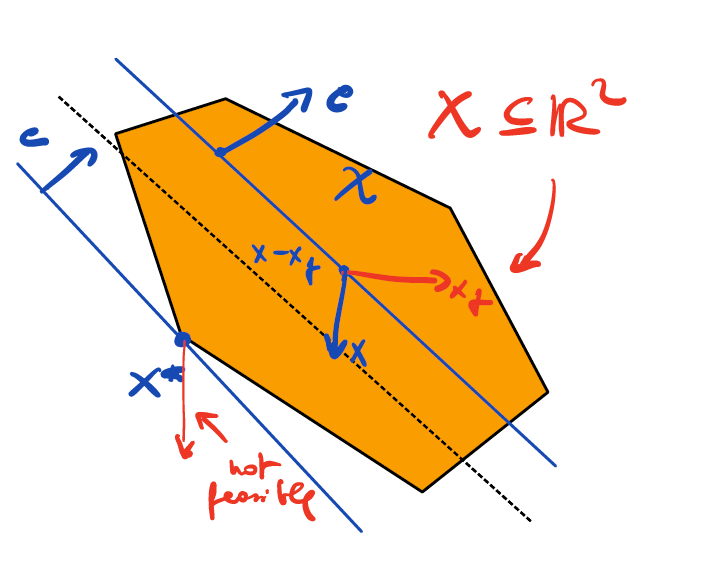
\includegraphics[scale=0.3]{img/LP_fig.png}
    \end{center}
    \newcolumn
    \textbf{Example(2): Max flow problem}
    \vspace{-0.2cm}
    \begin{quote}Maximize a certain quantity $f$, sent from a source to a sink, through a network represented by a digraph.\end{quote}
    - $C$ (matrix of capacities), $c_{ij}$ (link capacity from $i$ to $j$)\\
    - $X$ (matrix of effective flow) -- clearly $x_{ij} \le c_{ij}$\\
    - $\phi_{in} = \sum_{i=1}^n{x_{ik}}$, $\phi_{out}=\sum_{j=1}^n{x_{kj}}$\\
    \textbf{Constraints}   $\begin{cases}
        \phi_{in}-\phi_{out}=-f&\text{at source (node 1)}\\
        \phi_{in}-\phi_{out}=f&\text{at sink}\\
        \phi_{in}-\phi_{out}=0&\text{intermediate (node $n$)}
    \end{cases}$\\   
    \textbf{Objective} $\max_{x\in\mathbb{R}^n, f\in\mathbb{R}}{f} \iff -\min_{x\in\mathbb{R}^n, f\in\mathbb{R}}{-f}$
    \begin{center}
        $\begin{aligned}
            -p^*=&\min_{x\in\mathbb{R}^n, f\in\mathbb{R}} -f\\
            &\text{s.t.} \ (X^T-X)\mathbf{1}=\begin{bmatrix}
                -f\\0\\f
            \end{bmatrix}, \ 0_{n\times{n}} \le X \le C
        \end{aligned}$
    \end{center}
\end{multicols}

\subsection*{\underline{10. Second-order cone programs (SOCP)}}
\textbf{Second order cone} $\mathcal{K}_p=\{(u,t): \ u\in\mathbb{R}^{p-1}, \ t\in\mathbb{R}, \Vert u \Vert_2\le{t}\}$ extension of 
$\mathcal{K}=\{(x,y,z): \ \sqrt{x^2+y^2}\le{z}\}$\\
\textbf{$\mathbb{R}^n$-cone} $\mathcal{K}_n =\{x\in\mathbb{R}^n: \sqrt{x_2^2+x_3^2+...+x_n^2}\le{x_1}\}$\\
\textbf{Rotated cone} 
$\mathcal{K}_n^r\doteq\{x\in\mathbb{R}^n: \ x_3^2+x_4^2+...+x_n^2\le2x_1{x_2}, \ x_1, x_2 >0\}$\\
\textbf{Useful equivalence} $\Vert u \Vert_2^2 \le yz \ y\ge0, \ z\ge0 \iff \Vert \binom{2u}{y-z} \Vert_2 \le y+z$
\begin{multicols}{3}
    \noindent
    \textbf{Standard form for SOCP}
    \begin{center}
        $\begin{aligned}
            &\min_{x} c^T{x}\\
            &\text{s.t.} \ Ax=b, x^i \in \mathcal{K}_{n_i}
        \end{aligned}$
    \end{center}
    $x^i$ is the $i$-th block of the decision variable, $n_i$ its dimension.
    \newcolumn\\
    \textbf{SOC constraints}\\
    Given $u= Ax+b$, $t=c^T{x}+d$\\

    $\mathcal{K}=\{x: \Vert Ax+b \Vert_2 \le c^T{x}+d\}$
    \begin{center}
    \end{center}
    \newcolumn
    I can rewrite the problem as:
    \begin{center}
        $\begin{aligned}
            &\min_{x} {c^T{x}}\\
            &\text{s.t.} \ \Vert A_i{x}+d_i \Vert_2 \le c_i^T{x}+b_i
        \end{aligned}$
    \end{center}
    \hrule
    SOCP class encapsulate also the Linear and Quadratic programs.
\end{multicols}
\begin{multicols}{4}
    \noindent
    \textbf{LP as SOCP $\Longrightarrow$}
    \begin{center}
        $\begin{aligned}
            &\min_{x} c^T{x}\\
            &\text{s.t.} \ a_i^T{x}\le{b_i}, \ i=1,...,m
        \end{aligned}$
    \end{center}
    \newcolumn
    \text{problem transformation}
    \begin{center}
        $\begin{aligned}
            &\min_{x} c^T{x}\\
            &\text{s.t.} \ \Vert C_i{x}+d_i \Vert_2 \le b_i-a^T{x}\\
            &C_i=0, d_i=0, \ i=1,...,m
        \end{aligned}$
    \end{center}
    \newcolumn
    \textbf{QP as SOCP $\Longrightarrow$}
    \begin{center}
        $\begin{aligned}
            &\min_{x} x^T{Q}x+c^T{x}+d\\
            &\text{s.t.} \ a_i^T{x} \le b_i, \ i=1,...,m
        \end{aligned}$
    \end{center}
    \newcolumn
    \text{problem transformation}
    \begin{center}
        $\begin{aligned}
            &\min_{x,y} {c^T{x}+y}\\
            &\text{s.t.} \ \bigg\Vert\binom{2Q^{1/2}}{y-1} \bigg\Vert_2 \le y+1 \\
            &\text{s.t.} \ a_i^T{x} \le b_i, \ i=1,...,m
        \end{aligned}$
    \end{center}
\end{multicols}
\noindent
\textbf{Sum of Norms (SON)} $\min_{x} \sum_{i=1}^p \Vert A_i x - b_i\Vert_2 \longrightarrow 
\min_{x,y} {\sum_{i=1}^p{y_i}} \ \text{s.t.} \  \Vert A_i x - b_i\Vert_2 \le y_i, \ i=1,...,p$, $y_i$ slack variables\\
\textbf{Max of Norms} $\min_{x} \max_{i=1,...,p} \Vert A_i{x}-b \Vert_2$ $\longrightarrow$ $\min_{x,y} y \ \text{s.t.} \
\Vert A_i{x}-b \Vert_2 \le y, \ i=1,...,p$\\

\begin{multicols}{2}
    \noindent
    \textbf{Example(1): Fermat-Weber Point}
    \begin{quote}
        Where to locate a warehouse in order to serve in the best way some location services?
    \end{quote}
    $x\in\mathbb{R}^2$: position of the warehouse\\
    $y_i\in\mathbb{R}^2, \ i=1,...,m$: position of the location services\\
    I have to solve: $\min_{x}\frac{1}{m} \sum_{i=1}^m {\Vert{x-y_i}\Vert_2}$ (use SON)
    \begin{center}
        $\underbrace{\begin{aligned}
            &\min_{x,t} \frac{1}{m} \sum_{i=1}^m{t_i}\\
            &\text{s.t.} \ \Vert x-y_i \Vert_2 \le t_i, \ i=1,..., m
        \end{aligned}}_{\text{SOC Program}}$
    \end{center}    
    \newcolumn 
    \textbf{Example(2): LP with probability constraints}
    \begin{quote}
        How to solve an LP problem when one or more data are random or uncertain?
    \end{quote}
    In particular: \\
    -$a_i$ random normally distributed vectors $\begin{cases}
        \mathbb{E}\{a_i\}=\bar{a}_i\\
        \text{var}(a_i)=\Sigma_i\succ0
    \end{cases}$\\
    -$a_i^T{x}$ is a random variable $\to$ ($\mu=\bar{a}_i^T{x}, \ \sigma^2=x^T\Sigma_i{x})$, 
    -We know a-priori $P\{a_i^T{x}\le{b_i}\}\ge{p_i}, i=1,...,m$\\
    If $p_i>0.5$ the LP problem can be rewritten as: 
    \begin{center}
        $\underbrace{\begin{aligned}
            &\min_{x} {c^T{x}}\\
            &\text{s.t.} \ \bar{a}_i^{T}{x}\le b_i - \Phi^{-1}(p_i)\Vert \Sigma_i^{1/2}{x}\Vert_2
        \end{aligned}}_{\text{SOC Program}}$
    \end{center}
\end{multicols}
\vspace{-0.8cm}
\subsection*{\underline{11. CVX modeling}}
\begin{multicols}{2}
    \noindent
Example (LP Program)
\begin{verbatim}
cvx_begin [quiet]
    cvx_solver mosek        
    variable(s) x(2)    % name(dimension)
    minimize (c'*x)     %objective function
    subject to             
        A*x <= b;       %constraints
cvx_end 
\end{verbatim}
    \newcolumn
    You can write the problem also in a non-standard form, \texttt{cvx} will recast the problem in a standard form. \\
    Variables: $\begin{cases}
        \texttt{x}&\text{the minimizer}\\
        \texttt{cvx\_optval}&\text{the value} \ p^*\\
        \texttt{cvz\_status}&\texttt{Solved, Unfeasible, Unbounded}
    \end{cases}$\\

    \noindent
    useful function: \texttt{quad\_form(x,Q)}, returns $x^T{Q}x$ if $Q\succ0$
\end{multicols}
\subsection*{\underline{12. General optimization and Lagrangian Duality}}
\textbf{Langrangian} $\mathcal{L}(x,\lambda, \nu)=f_0(x)+\sum_{i=1}^m{\lambda_i{f_i(x)}}+\sum_{i=1}^p{\nu_i{h_i(x)}}$ -- $\lambda_i, \ \nu_i$ \textbf{Lagrange multipliers} -- $f_0(x)\ge\mathcal{L}(x,\lambda,\nu)$\\
\textbf{Lagrangian dual function} $g(\lambda, \nu) = \underset{x\in\mathcal{D}}{\text{inf}} \ {\mathcal{L}(x, \lambda, \nu)}, \ \lambda>0$, \ $g:\mathbb{R}^m\times\mathbb{R}^p\to\mathbb{R}$ -- \textbf{Properties} $\begin{cases}
    \text{jointly concave in} (\lambda,\nu)\\
    g(\lambda,\nu)\le p* \ \forall \lambda>0, \forall \nu
\end{cases}$\\
\textbf{Dual problem} (What is the best $g(\lambda,\nu)$)? $d^*=\max_{\lambda,\nu} g(\lambda,\nu) \ \text{subject to}: \lambda>0 $ -- $d^*\le{p^*}$ (\textbf{...is always convex})\\
\textbf{Duality gap} $\delta^*=p^*-d^*=\begin{cases}
    =0&\text{strong duality (further conditions are needed)}\\
    >0&\text{weak duality}
\end{cases}$\\
\textbf{Slater's condition for STRONG DUALITY} Let $f_i(x)$ convex functions, $h_i(x)$ affine functions, $f_i(x), i=1,...,k\le{m}$ affine, if $\exists{x}\in\text{relint}\ \mathcal{D}$: $f_i(x)\le0, \ i=1,..., k$, $f_{k+1}(x)<0, ..., f_m(x)<0$, $h_i(x)=0, \ i=1,...,p$ then: $p^*=d^*$ (there is no gap), moreover if the problem is not unbounded below $\exists(\lambda^*,\nu^*): \ g(\lambda^*, \nu^*)=d^*=p^*. $\\
\vspace{-0.8cm}
\begin{multicols}{2}
    \noindent
    \textbf{Primal problem}
    \vspace{-0.2cm}
    \begin{equation*}
        p^*=\min_{x} \max_{\lambda,\nu} \mathcal{L}(x,\lambda,\nu)
    \end{equation*}
    \newcolumn\\
    \textbf{Dual problem}
    \vspace{-0.2cm}
    \begin{equation*}
        d^*=\max_{\lambda,\nu} \min_{x} \mathcal{L}(x,\lambda,\nu)
    \end{equation*}
\end{multicols}
\vspace{-0.6cm}
\noindent
\textbf{Primal solution from dual solution} (Required: strong duality) $d^*=p^*=f_0(x^*)$, $d^*=g(\lambda^*,\nu^*)=\mathcal{L}(x,\lambda^*,\nu^*)$  \\
$f_0(x^*)=\mathcal{L}(x^*,\lambda^*,\nu^*)=f_0(x^*)+\sum_{i=1}^m {\lambda_i}^*f_i(x^*) + \sum_{i=1}^p \nu_i^*{h_i(x^*)}\to$
$\begin{cases}
    \sum_{i=1}^m {\lambda_i}^*f_i(x^*)=0&\textsf{complementary slackness}\\
    x^*&\textsf{minimizer (wrt $x$) of} \ {\small{\mathcal{L}(x,\lambda^*,\nu^*)}}
\end{cases}$\\
\textbf{\small Complementary slackness} For the $i$-th constraint: either $\lambda_i=0, f_i(x)\le0$, or $\lambda_i>0, f_i(x)=0$\\
\textbf{\small Solution recovery} If $f_0$ convex, $\nabla_x \ {\mathcal{L}(x,\lambda^*, \nu^*)}=0$ gives a \textbf{global minimizer} (unique  if $f_0$ strictly convex).\\
$\underset{f_0 \ \text{differentiable, strong duality holds.}}{\textbf{KKT conditions for optimality} \text{(optimal $\iff \ \delta^*=0$)}}$    $\begin{cases}
    \textsf{1. primal feasibility}&f_i(x^*)\le0, \ h_i(x^*)=0 \\
    \textsf{2. dual feasibility}&\lambda_i^*\ge0, \ i=1,...,m\\
    \textsf{3. complementary slackness}&\sum_{i=1}^m {\lambda_i^*}f_i(x^*)=0\\
    \textsf{4. Lagrangian stationarity}&\nabla_x \ {\mathcal{L}(x,\lambda^*, \nu^*)}\big|_{x=x^*}=0\\
\end{cases}$\\
\textbf{Sensitivity of the optimal solution $p^*$}
\vspace{-0.3cm}
\begin{multicols}{2}
    \noindent
    \textbf{\small Perturbed Problem}
    \vspace{-0.2cm}
    \begin{align*}
        p^*(u,v) =& \min_{x\in\mathbb{R}^n} f_0(x)\\
        &\text{s.t.} \ f_i(x)\le{u_i},\ h_i(x)=v_i
    \end{align*}
    \textbf{Remark:} $p^*(0,0)=p^*$ --
    $u_i>0\to$ relaxing, $u_i<0$ tightning. 
    When the primal problem is convex and $p^*(u,v)$ differentiable: 
    \begin{align*}
        \lambda_i^* = -\frac{\partial{p^*(u,v)}}{\partial{u_i}}\big|_{(u,v)=(0,0)}, \ 
        \nu_i^* = -\frac{\partial{p^*(u,v)}}{\partial{v_i}}\big|_{(u,v)=(0,0)}
    \end{align*}
    \textbf{Interpretation:} {\tiny{(here I use the complementary slackness)}} \\
    $\lambda_i^*=0 \Rightarrow f_i(x^*)<0$ the constraint is inactive, I don't care about perturbations $\to$ not resource critical! \\$\lambda_i^*>0 \Rightarrow f_i(x^*)=0$ constraint active (resource critical) $\to {p^*_{new}=p^*-\lambda_i^*{u_i}}$.\\
    In particular: $\begin{cases}
        u_i<0&p^* \ \text{increase (worse solution)}\\
        u_i>0&p^* \ \text{\textbf{can} decrease (better solution)}
    \end{cases}$\\

    \noindent
    Remember that: the Lagrange multipliers are given by the solution of the dual problem.
\end{multicols}
\newpage

\subsection*{\underline{13. Gradient Algorithm (GA)} (\textsf{unconstrained case})}
\vspace{-0.3cm}
\begin{multicols}{2}
    \noindent
    \textbf{General structure: } $x_{k+1}=x_k + s_k{v_k}$\\
    $s_k>0, \ s_k \in \mathbb{R}$ (step-size)\\
    $v_k\in\mathbb{R}^n$ (update/search direction)\\
    For Gradient Algorithm: $\begin{cases}
        f_0 \ \text{differentiable}\\
        x_k \in \text{dom}(f_0)\\
        v_k \in \mathbb{R}^n \text{(chosen wrt $\nabla{f_0(x)}$)} 
    \end{cases}$
    $f_0:\mathbb{R}^n\to\mathbb{R}$, $f_0(x_k+s{v_k})\simeq{f_0(x_k)}+s\nabla{f_0(x_k)}^T{v_k}$\\
    $t\to\infty$, $\delta_k=\lim_{s\to\infty}{\frac{f_0(x_k+sv_k)-f_0(x_k)}{s}}=\nabla{f_0}(x_k)^T{v_k}$\\
    I want a direction for which $f_0$ decrease (descent). $\forall{k}$ moving toward $v_k$ $\to$ go to min.\\
    \textbf{Steepest descent direction:} $v_k=-\frac{\nabla{f_0}(x)}{\Vert f_0(x) \Vert_2}$
    \begin{algorithm}[H]
        \caption{Gradient Algorithm}
        \begin{algorithmic}[1]
            \State{$k=0$, choose a descent $v_k$ ($v_k=-\nabla{f_0(x_k)}$)}
            \State{\underline{Determine the step-size} $s_k$}
            \State{$x_{k+1}=x_k+s_k{v_k}$}
            \If{\underline{Stop criterion}} 
                \State{\Return{ $x_k$}}
            \Else 
                \State{back to 2}
            \EndIf
        \end{algorithmic}
    \end{algorithm}
    \vspace{-0.3cm}
    \noindent
    \textbf{\underline{STEPSIZE SELECTION}} $\overbrace{\phi(s)=f_0(x_k+s{v_k}), s\ge0}^{\text{restriction of $f_0$ along $v_k$}}$\\
    $\phi(0)=f_0(x_k)$, I want $s>0: \ f(x_{k+1})=\phi(s)<\phi(0)$\\
    \textbf{Exact line-search (best $s$ possible)} (non-convex)
    \vspace{-0.3cm}
    \begin{equation*}
        s^* = \arg\min_{s\ge0}{\phi(s)}
    \end{equation*}
    \begin{multicols}{2}
        \vspace{-0.5cm}
        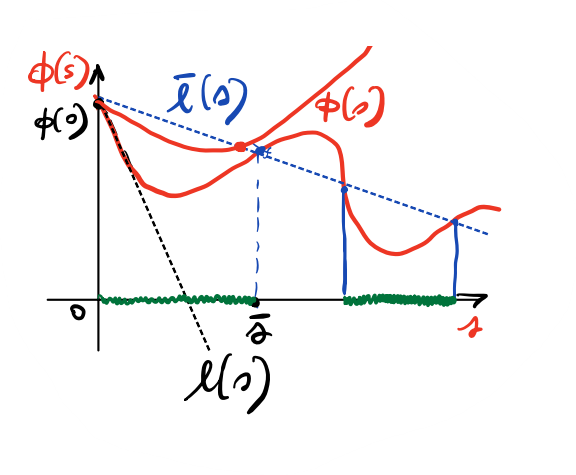
\includegraphics[scale=0.3]{img/gradient_1.png}
        \newcolumn\\
        $\ell(s)=\phi(0)+s\delta_k$ (tan at 0)\\
        $\bar{\ell}(s)=\phi(0)+\alpha{s\delta_k} $\\
        $\bar{\ell}(s)\ge \ell(s) \ge \phi(s)$\\
        $s: \ \phi(s)\le\bar{\ell(s)}$ are OK\\

        \noindent 
        \textbf{Armijo condition}\\
        $\phi(s)\le\phi(0)+s\alpha\delta_k$
    \end{multicols}
    \vspace{-1.5cm}
    \newcolumn
    \begin{algorithm}[H]
        \caption{Backtracking line-search}
        \begin{algorithmic}[1]
            \State{$\alpha\in(0,1), \ \beta\in(0,1), s_{init}=1, \ v_k$ descent}
            \If{$f_0(x_k+s{v_k})\le{f(x_k)}+s\alpha\nabla{f_0(x_k)}^T{v_k}$}
                \State{\Return{$s_k \ \gets \ s$}}
            \Else 
                \State{$s=\beta{s}$, back to 2} \Comment{\small{update until not Armijo's meet}}
            \EndIf
        \end{algorithmic}
    \end{algorithm}
    \vspace{-0.3cm}
    \noindent
    \textbf{\underline{CONVERGENCE OF GA: STOPPING CRITERION}}
    {\small $\nabla{f_0(x)}, \exists{L}: \Vert \nabla{f_0(y)}-\nabla{f_0(x)} \Vert_2 \le L\Vert y-x \Vert_2, \forall{x,y}$} {\small{(Lipschitz)} }\\
    $\Rightarrow$ $f_0(x) \le \underbrace{f_0(y) + \nabla{f_0(x)}^T(x-y)+\frac{L}{2}\Vert x-y \Vert_2}_{\text{strongly cvx, quadratic approximant}}$
    \begin{multicols}{2}
        \noindent
        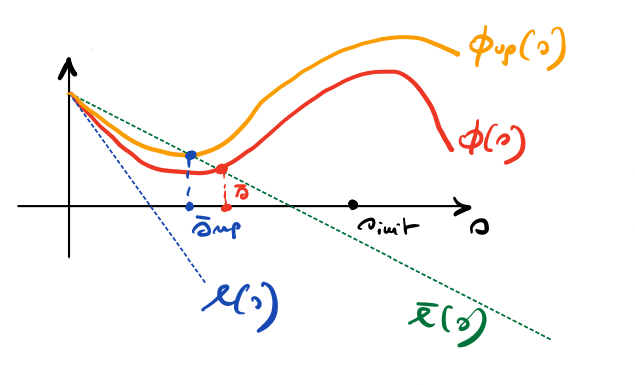
\includegraphics[scale=0.3]{img/gradient_2.png}
        \newcolumn\\
        I can introduce $\phi_{up}(s)$ since $\nabla{f_0}$ is Lipschitz. $\bar{s}_{up}\to$ intersection $\phi_{up}(s)$-$\bar{\ell(s)}$\\
        $\bar{s}_{up}=\frac{2}{L}(1-\alpha)$\\

        \noindent
        Backtracking ensures:\\
        {\small $\forall{k}, s_k\!\ge\!\min(s_{init}, \beta\bar{s}_{up})\doteq{s_{\text{lb}}}$}
    \end{multicols} 
    \vspace{-0.6cm}
    \noindent
    It holds that (GA converges to a stationary point):\\
    $\alpha{s_{\text{lb}}}\sum_{i=0}^k {\Vert \nabla{f_0}(x_i) \Vert_2^2} \le f_0(x_0)-f_0^*$,  
    $\underset{k\to\infty}{\lim}{\Vert \nabla{f_0}(x_i) \Vert_2}=0$\\
    \textbf{Stopping criterion} $\to \ \Vert \nabla{f_0}(x) \Vert_2 < \varepsilon, \varepsilon>0$\\
    $f_0$ convex $\to$ $x^*$ is a global minimizer.\\
    $\underset{\Vert \nabla{f_0(x_k)} \Vert_2 \to 0}{\textbf{Convergence}}$ $\begin{cases}
        O(1/\sqrt{k})&f_0 \ \text{generic}\\
        O(1/\varepsilon)&f_0 \ \text{convex (sublinear)}\\
        O(1/\log(1/\varepsilon))&f_0 \ \text{strongly convex (linear)}
    \end{cases}$\\
    \hrule\noindent
    \textsf{\textbf{Grad. Algorithm as minimization of $q(x)$}}\\
    GA can be interpreted also as minimization of the quadratic approximant when $\Vert x-x_k \Vert_2$ is small $\to$ $f_0(x)\simeq{q(x)=f_0(x_k) + \nabla{f_0(x_k)}^T(x-x_k)}$\\
    $\nabla{q(x)}\!=\!\nabla{f_0(x_k)}+\frac{1}{s}(x-x_k)=0 \Leftrightarrow\underset{\text{Gradient Algorithm}}{x_{k+1}=x_k-s\nabla{f_0(x_k)}}$\\
    \textbf{Conclusion:} $x$ is updated $\forall{k}$ by minimizing $q(x_k)$. $\square$
 \end{multicols}
\vspace{-1.1cm}
\noindent
\rule{\textwidth}{1.5pt}

\subsection*{\underline{14. Newton Algorithm (NA)} (\textsf{unconstrained case})}   
\vspace{-0.3cm}
\begin{multicols}{2}
    \noindent
    \textbf{Key concept:} Finding (starting from $x_k$) the roots of a non linear function $g:\mathbb{R}\to\mathbb{R}$. We want the roots of $\nabla{f_0(x)}=0$.\\
    $\tilde{g}(x)=g(x_k)+g'(x_k)(x-x_k)$. $x_{k+1}$ is given by $\tilde{g}(x)=0$
    \begin{equation}
        \overbrace{x_{k+1} = x_k - \frac{g(x_k)}{g'(x_k)} = x_k - (\nabla^2{f_0(x_k)})^{-1}\nabla{f_0(x_k)}}^{\textsf{NEWTON METHOD}} \label{eq:NM}
    \end{equation}
    {\small{$\underbrace{q_0(x)\!=\!f(x_k)\!+\!\nabla{f_0(x)}^T\!(x-x_k)\!+\!\frac{1}{2}(x-x_k)^T\nabla^2{f_0(x_k)}\!(x-x_k)}_{\text{quadratic approximant of $f_0$}}$}}
    \raggedcolumns
    \begin{multicols}{2}
        \noindent
        \begin{center}
            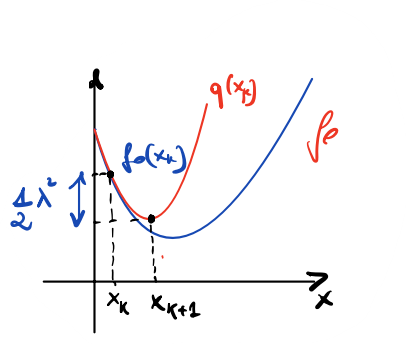
\includegraphics[scale=0.35]{img/newton.png}
        \end{center}
        $\arg\min_{x} q_0(x)=x_{k+1}\\
        \min_{x} {q_0(x)}=f(x_{k+1})$\\
     $\min_{x}{q_0(x)}-f(x)=\frac{1}{2}\lambda^2(x)$\\ 
     $\underbrace{\lambda^2=\nabla{f_0}^T\nabla^2{f_0}^{-1}\nabla{f_0}}_{\text{Newton decrement}}$\\
     where $\nabla{f_0} \leftrightarrow \nabla{f_0(x_k)}$
    \end{multicols}
    \noindent
     \textbf{Damped Newton Method}  $x_{k+1}=x_k+tv$\\
     $v\!=\!-\nabla^2{f_0(x_k)}^{-1}\nabla{f_0(x_k)}$,\! $\nabla{f_0(x_k)}^T\cdot{v}\!=\!\!-\!\lambda^2\!<\!0$ \!(\textbf{descent})
     \vspace{0.05cm}
     \begin{algorithm}[H]
        \caption{Choice of $t$ (step-size) }
        \begin{algorithmic}[1]
            \State{$\alpha \in (0,\frac{1}{2}], \ \beta \in (0,1), t=1$}
            \While{$f_0(x_k+tv) > f(x_k) + \alpha{t}\nabla{f_0(x_k)}^T{v}$}
                {$t \ \gets \ t \beta$}
            \EndWhile
            \State{$x_{k+1} = x_k + tv$}
        \end{algorithmic}
     \end{algorithm}
     \vspace{-0.5cm}
     \noindent
     \textbf{Convergence properties} $f_0$ strongly convex, $\nabla{f_0}, \nabla^2{f_0}$ Lipschitz continuous, $\eta \in (0, m^2/L)$. \\
     2 phases:
     $\begin{cases}
        \Vert \nabla{f_0(x_k)} \Vert \ge \eta&\text{Damped phase}\\
        \Vert \nabla{f_0(x_k)} \Vert < \eta&\text{Quadratically convergent phase}
     \end{cases}$\\
     \textbf{Stopping criterion} $f_0(x_k) - f_0^* \le \lambda_k^2$\\
     \textsc{\underline{Other aspects (1): Equality constraints}}\\
     I choose $x_0: Ax_0=b$, and $x_{k+1}=x_k+tv$, where
     \vspace{-0.2cm}
     \begin{equation*}
        \small
        v=\arg\min_{z\in\mathcal{N}(A)} {\!\nabla{f_0(x)}^T\!(z-x)\!+\!\frac{1}{2}(z-x)^T\nabla^2{f_0(x_k)}\!(z-x)}
     \end{equation*}
     In this way, since $A{x_{k+1}}=A{x_{k}}+tAv=b$, $x_k$ remains in the feasible set, $Av=0$.\\
     \noindent
     \textsc{\underline{Other aspects(2): QUASI-NEWTON methods}} \\
     \textbf{Secant condition} $H(\nabla{f(x)}-\nabla{f(y)})=(x-y)$ $\Rightarrow$ a matrix $H$ satisfying such a condition can approximate the Hessian.

     \begin{algorithm}[H]
        \caption{Quasi-Newton methods}
        \begin{algorithmic}[1]
            \State{$H_k=I_n$}
            \State{Update s.t.: $H_{k+1}\nabla{f_0(x_{k+1})}-\nabla{f_0(x_k)}=x_{k+1}-x_k$}

        \end{algorithmic}
     \end{algorithm}
     
\end{multicols}

\subsection*{\underline{15. Approaches for constrained optimization}}
\begin{center}
    \textsf{When there are constraints solving $\nabla{f_0(x)}=0$ it is not sufficient, $x^*$ must be feasible and $\mathcal{X}\ne\mathbb{R}^n$}
\end{center}
\vspace{-0.2cm}
\textbf{1$^{st}$ approach: \textit{Projected Gradient Method}}
\vspace{-0.3cm}
\begin{multicols}{2}
    \noindent
    $\mathcal{P}_\mathcal{X}(x)$ $\leftarrow$ projection of $x$ on the feasible set $\mathcal{X}$ (convex, non-empty). 
    \vspace{-0.3cm}
    \begin{algorithm}[H]
        \caption{Projected Gradient Method}
        \begin{algorithmic}[1]
            \State $k=0$
            \State $w_{k+1}=x_{k}-s_k\nabla{f_0(x_k)}$  \Comment{Gradient Step}
            \State $x_{k+1}=\mathcal{P}_\mathcal{X}(w_{k+1})$ \Comment{ensure feasibility}
        \end{algorithmic}
    \end{algorithm}
    \vspace{-0.5cm}
    \noindent
    (used only for set for which is simple to compute projections, otherwise other more general methods are used).
    \newcolumn\\
    The $s_k$ (step-size) is chosen as follows: $s_k=\bar{s}2^{-t(k)}$
    \vspace{-0.3cm}
    \begin{algorithm}[H]
        \caption{Stepsize selection}
        \begin{algorithmic}[1]
            \State{$j=0$}
            \State{$z_j=\mathcal{P}_{\mathcal{X}}(x_k-\bar{s}{2^{-j}}\nabla{f_0(x_k)})$}
            \If{$f(z_j)\le{f(x_k)}-\alpha\nabla{f_0(x_k)}^T(x_k-z_j)$}
                \State $t(k)=j$
            \Else
                \State goto 2
            \EndIf
        \end{algorithmic}
    \end{algorithm}
    \noindent
\end{multicols}
\vspace{-0.2cm}
\noindent
\rule{\textwidth}{1.3pt}
\noindent
\textbf{$2^{nd}$ approach: \textit{Barrier Method}}
\vspace{-0.4cm}
\begin{multicols}{2}
    \noindent
    Here we want to solve ($f_0, ..., f_m$ convex and smooth): 
    \vspace{-0.2cm}
    \begin{align*}
        p^*=&\min_{x}  f_0(x)\\
        &\text{s.t.} \ f_i(x)\le0, \ i=1,...,m\\
        &Ax=b 
    \end{align*}
    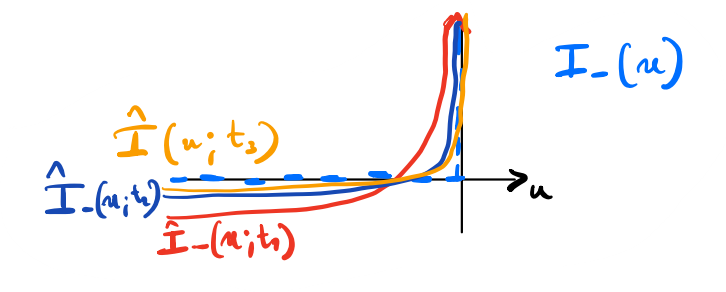
\includegraphics[scale=0.4]{img/barrier.png}\\
    The problem can be rewritten as: 
    \vspace{-0.3cm}
    \begin{align}
        &p^*=\min_{x} f_0(x)+\sum_{i=1}^{m} {I_{-}(f_i(x))}\label{eq:prob_ind}\\ 
        &I_{-}(u)=\begin{cases}
            0&{u}\le0\\
            \infty&u>0
        \end{cases} \quad \textsf{(Indicator function)}
    \end{align}
    \vspace{-0.3cm}
    $I_{-}(u)$ non-differentiable $\to$ ${\hat{I}_{-}(u;t)=-\frac{1}{t}\log(-u)}$
    \begin{align}
        p^*(t)&=\min_{x} f_0(x)\overbrace{-\frac{1}{t}\sum_{i=1}^{m} {log(-f_i(x))}}^{\phi(t) \to \textbf{logarithmic barrier}}=\\
        &=\min_{x} {t{f_0(x)}+\phi(t)}\label{eq:barrier} \\ 
        &\text{s.t.} \ Ax=b
    \end{align}
    Parametrizing the $x$, (\ref{eq:barrier}) becomes unconstrained (GA, NM can be used).\\
    \noindent
    For $t\to\infty$ (\ref{eq:barrier})$\to$(\ref{eq:prob_ind}) that is
    $p^*(t)\to{p^*}, \
        x^*(t)\to{x^*}$\\
    \textbf{Central path}$\{x^*(t):t>0\}$, $p^*(t)$ $\varepsilon$-suboptimal
    $\varepsilon=m/t$
    \vspace{-0.5cm}
    \begin{algorithm}[H]
        \caption{Sequential Barrier Method}
        \begin{algorithmic}[1]
            \State{$x_0$ (strictly feasible), $t{\gets}t_0$, $\mu>1$, $\varepsilon>0$}
            \Loop{}
                \State Solve $\min_{Ax=b}{tf_0(t)+\phi(t)}$ \Comment{Centering step}
                \State $x{\gets}x^*(t)$
                \If{$m/t<\varepsilon$}  \Comment{Stopping criterion}
                    \State \textbf{break}
                \Else  \State{$t \gets \mu{t}$} \Comment{Increase $t$ (better approx of $I_{-}(u)$)}
                \EndIf
            \EndLoop
        \end{algorithmic}
    \end{algorithm}
    \vspace{-0.3cm}
    \noindent
    \textbf{\underline{Phase I Problem}: starting from a feasible $x_0$} 
    \vspace{-0.3cm}
    \begin{multicols}{2}
        \begin{align*}
            \tilde{s}=&\min_{x,s} {s}\\
            &\text{s.t.} \ f_i(x)\le{s}, \\
            &Ax=b
        \end{align*}
        \newcolumn\\
        Solved by using the barrier method, starting from:\\
        $x_0: \ Ax_0=b$,    \\
        $s_0=\eta+\max_{i}{f_i(x)}, \ \eta>0$
    \end{multicols}
    \vspace{-0.8cm}
    \hrule
    \vspace{0.1cm}
    \noindent
    $\to$ $\tilde{s}<0$. Since $f_i(\tilde{x})\le\tilde{s}\le0 \longrightarrow x_0=\tilde{x}$\\
    $\to$ $\tilde{s}>0$. $\nexists{x}: \ f_i(x)\le0$ $\longrightarrow$ problem infeasible\\
    $\to$ $\tilde{s}=0$. Only of theoretical interest\\

    \noindent
    \textbf{Remark:} For carrying out the \textit{centering step} the \textsc{Newton Method} tailored for equality constraints is used.
\end{multicols}
%\newpage

\subsection*{\underline{16. Geometric Programs(GP)}}
For GP: \textbf{variables} $\to$ positive (physical quantities), \textbf{objective/constraints} $\to$ non-negative linear combination of positive monomials.\\
\textbf{Positive monomial} Given $x\in\mathbb{R}^n,\ a \in \mathbb{R}^n, \ c>0, x>0$ $cx^a=cx_1^{a_1}x_2^{a_2}...x_n^{a_n}\in\mathbb{R}^+$\\
\textbf{Posynomial} $f:\mathbb{R}^n_{++}\to\mathbb{R}$, $f(x)=\sum_{i=1}^{k}{c_i x^{a_{(i)}}}, \ c_i, x>0, a_{(i)}\in\mathbb{R}^n$ -- $\underset{\textsf{composite fun. of posynomials}}{\textbf{Generalized posynomial}} \begin{cases}
    \text{pointwise maximum}\\
    \text{fractional power}\\
    \text{addition/multiplication}
\end{cases}$\\
Monomials, Posynomials and Generalized posynomials \textbf{are not convex!} $\to$ \underline{Problem transformation is needed}\\
\textbf{Convex form for monomials} $y_i=\log x_i$ $\to \ \tilde{g}(x)=cx_1^{a_1}...x_n^{a_n}=e^{\log c}e^{\log{x_1^{a_1}}}...e^{\log{x_n^{a_n}}}=e^{a_1{y_1}+...+a_n{y_n}+\log{c}}=e^{a^T{y}+b}$. I can take the log (f convex $\circ$ f increasing) obtaining $g(x)=\log{\tilde{g}(x)}=a^T{y}+b$ $\to$ Linear Program\\
\textbf{Convex form for posynomials} $\tilde{f}(x)=\sum_{i=1}^{k}{c_i{x}^{a_{(i)}}}=\sum_{i=1}^{k}{e^{a_{(i)}^T{y}+b_i}}\to
\tilde{y}(x)=\log\bigg({\sum_{i=1}^{k}{e^{a_{(i)}^T{y}+b_i}}}\bigg)=\text{lse}(Ax+b)$\\
log-sum-exp (lse) function is convex -- $A\in\mathbb{R}^{k,n}, \ b = [b_1 \quad \dots \quad b_n]^T$\\
\newpage

\noindent
\textbf{Standard form for GP} Here $f_0(x), f_i(x)$ are posynomials, $h_i(x)$ are (possibly) monomials
\vspace{-0.3cm}
\begin{multicols}{2}
    \begin{align*}
        &\min_{x} {\sum_{k=1}^{K_0}{c_k{x^{a_{(k)}}}}}\\
        &\text{s.t.} \ \sum_{k=1}^{K_i}{c_k}x^{a_{(k)}} \le 1, \ i=1,...,m\\
        &g_i{x^{r_{(i)}}}=0, \ i=1,...,p
    \end{align*}
    \newcolumn\\
    \textbf{Geometric programs in standard form}
    \begin{align*}
        &\min_{y} \text{lse}(A_0y+b_0)\\
        &\text{s.t.} \ \text{lse}(A_i{y}+b_i)\le0\\
        &Ry+h=0\\
        &A_0\in\mathbb{R}^{K_0,n}, b_0 \in \mathbb{R}^{K_0}, \ A_i\in\mathbb{R}^{K_i,n}, b_0 \in \mathbb{R}^{K_i}
    \end{align*}
\end{multicols}
\noindent
\textbf{Generalized GP} $f_0, ..., f_m$ are generalized posynomials $\to$ GGP (Generalized GP)\\
{\small{\textbf{Fractional power}}} $f_1(x)^\alpha + f_2(x)^\beta\le1 \Rightarrow \underbrace{f_1(x)\le{t_1}, \ f_2(x)\le{t_2}, \ t_1^\alpha+t_2^\beta\le1}_{\text{GP constraints}}$  \\
{\small{\textbf{Pointwise maximum power}}} $\max(f_1(x), f_2(x))+f_3(x)\le1 \Rightarrow 
\underbrace{f_1(x)\le{t}, f_2(x)\le{t}, t+f_3(x)\le1}_{\text{GP constraints}}$ \\

\noindent
\subsection*{\underline{APPENDIX}}
\textbf{Schur complement} $M=\begin{bmatrix}
    A&X^T\\
    X&B
\end{bmatrix}, A,B\in\mathbb{S}^n \ M\succeq0 \  \iff S=A-XB^{-1}X^T\succeq0$  \\
\textbf{Young inequality} If $a\ge0$, $b\ge0$, $p>1$, $q>1$ such that $\frac{1}{p}+\frac{1}{q}=1$ then $ab \le \frac{1}{p}{a^p}+\frac{1}{q}{b^q}$ \textsf{(Jensen's inequality can be used in order to demonstrate it)}\\
\textbf{Maxima of inner product over a ball} $\underset{\Vert x \Vert_p \le 1}{\max} x^Ty$ $\begin{cases}
    \max_{\Vert x \Vert_2\le1}{x^T{y}}=\Vert{y}\Vert_2, \ x^{*}=\frac{y}{\Vert{y}\Vert_2}&{p=2}\\
    \max_{\Vert{x}\Vert_\infty\le1}{x^T{y}}=\sum_{i=1}^{n}{\vert{y_i}\vert}=\Vert{y}\Vert, \ x^{*}_\infty=\text{sgn}(y)&{p=\infty}\\
    \begin{aligned}
        &\max_{\Vert{x}\Vert_1\le{1}}{x^T{y}}=\max_i{\vert{y_i}\vert}=\Vert{y}\Vert_\infty \\
        &[x_1^{*}]_i=\begin{cases}
           \text{sign}(y_i)&\text{if} \ i=m\\
           0&\text{otherwise}
       \end{cases}, \ i=1,...,n
    \end{aligned}&p=1
   
\end{cases}$


\end{document}